\frame{
\frametitle{Klassenstruktur}
    \begin{block}{Struktur}
    \begin{itemize}
        \item Erweiterung im \textbf{Parametrierungsskript} zum setzen der jeweiligen \textbf{Hochschule} über \textbf{Optionsmenü}
        \item \textbf{Spracheinstellungen} werden aus dem System übernommen
    \end{itemize}
        \begin{center}
            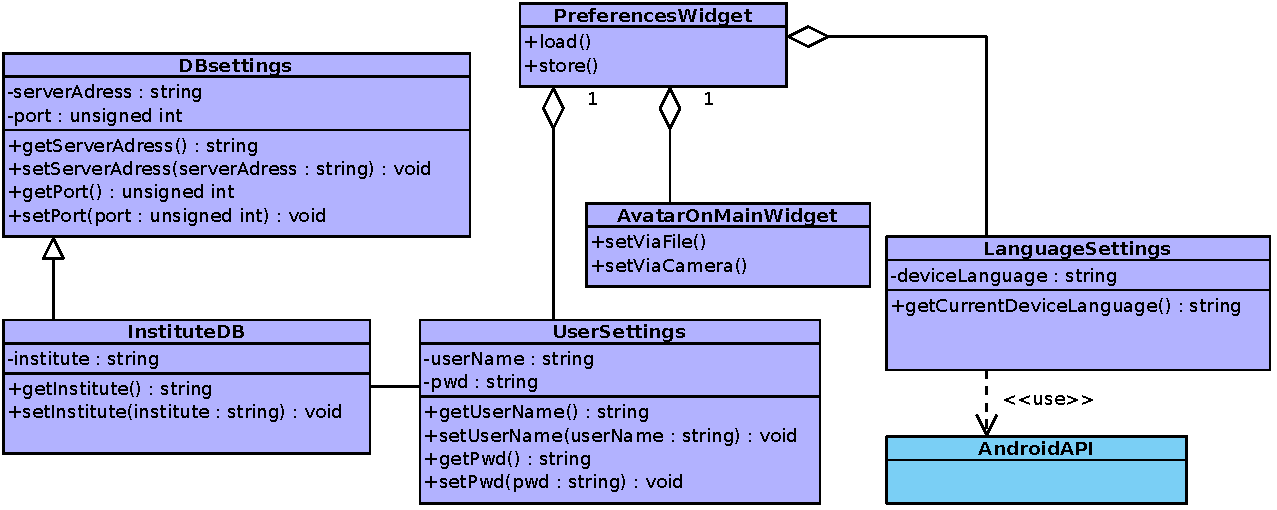
\includegraphics[width=0.8\textwidth]{../grafiken/OptionWidgetB.pdf}
        \end{center}
    \end{block}
}